\lfoot{Autor: Fitim Faiku}
\subsection{Android App}
<<<<<<< HEAD
Die Android App ist dazu da, um den Usern die Generierten Daten möglichst Aufschlussreich darzustellen.
Bei der Android App werden erstmal die drei Seiten(Tabs) erstellt. Die Tabs werden den drei Hauptfeauters zugeordnet(Verbrauchsanalyse-Fahrgastkommfort-Schaltvorschlag). 
=======
\label{subsec:androidapp}

>>>>>>> aca00159eb7a63f092a2c4b8c38e908b9a2a051b
Die Android App wurde mittels Java erstellt wobei als Programmieroberfläche Android Studio verwendet wurde.
Für jede Klasse wurde ein XML Layout als View generiert, wodurch eine Verbindung zwischen Code und Layout geschaffen wurde.

\subsubsection{Code-Dokumetation}
 Um die Grafiken bestmöglich darzustellen und dabei eine möglichst hohe Anzahl an Usern zu erreichen, entschieden wir uns eine Android App zu entwickeln.
 Dabei achteten wir besonders auf die Benutzerfreundlichkeit der Applikation.
 Die wichtigsten Kriterien waren, dass der Fahrer im Straßenverkehr nicht abgelenkt wird, er sehr leicht zwischen den einzelnen Features wechseln kann und die Informationen intuitiv aufbereitet sind.
 
 Um die App zu realisieren erstellten wir mehrere Fragments zwischen denen man hin und her \textit{swipen} kann.
  Es wurde zuerst eine MainActivity Klasse erstellt, welche von FragementActivity erbt und von ActionTabListener implementiert, um die Methoden onTabReselected, onTabselected und onTabunselected zu überschreiben. 
\lstinputlisting[caption=Design-Beispiel, style=javastyle]{code/MyActivity.java}


  
 
            
Im Anschluss setzten wir die View der Klasse auf main durch:  

\lstinputlisting[firstline=1,lastline=1, style=javastyle, caption=Setzen der View]{code/examples.java}

Wir erstellten ein Objekt von ActionBar und fügten mehrere Tabs hinzu und setzten das Layout für die Navigation der Tabs mittels:

\lstinputlisting[firstline=2,lastline=2, style=javastyle, caption=ActionBar Objekt]{code/examples.java}

Anschließend wurden mehrere Tabs hinzugefügt mit der Methode:

\lstinputlisting[linerange={4-8}, style=javastyle, caption=Mehrere Tabs]{code/examples.java}


Nun gehen wir über zu unserem Design unter main.xml
\lstinputlisting[caption=Design main, style=xmlstyle]{code/main.xml}
Es wurde ein ViewPager Layout erstellt welches das \textit{swipen} möglich macht:

\lstinputlisting[firstline=10,lastline=10, style=xmlstyle, caption=Swipe Funktion]{code/examples.java}

Wir übergeben dem Layout ebenfalls eine ID auf die wir von unserer main Activity aus zugreifen: 
\lstinputlisting[firstline=12,lastline=12, style=xmlstyle, caption=Activity und Layout]{code/examples.java}



Es wird eine Fragementadapter-Klasse erstellt um die einzelnen Seiten den Klassen zuzuteilen. 
Die Klasse hat einen Konstruktor, welcher von der Superklasse das FragementManager Objekt übergeben bekommt.
Weiters hat die Klasse eine getItem Methode mit dem Input eines int Wertes. 
\lstinputlisting[caption=PageAdapter, style=javastyle]{code/FragementPageAdapter.java}


Es wird hierbei überprüft ob, welcher Tab aktiviert wurde, und der wird der entsprechenden Klasse eingeteilt. 
Sie hat noch eine getCount() Methode, welche die Anzahl der Tabs zurückgibt in unserem Fall drei für die Hauptfeauters.


Wir erstellen auf der Main Klasse zwei Objekte, nämlich:
\lstinputlisting[linerange={14-18}, style=javastyle, caption=Viewpager]{code/examples.java}

Dies wird gemacht um zwischen den Oberflächen wechseln zu können.

 

\subsubsection*{Implementierung von MPAndroidChart}
MPAndroidChart ist eine Libary mittels der 8 verschieden Graphen erzeugt werden können. Weiterhin sind Animationen mittels der Libary möglich, das bearbeiten von x und y Achsen und das abspeichern von Grafiken als image Files.

Das Liniendiagramm wurde mittels der MPAndroidChart Libary erstellt. Die Linien werden Blau gezeichnet und die einzelnen Punkte schwarz. Das Liniendiagramm wurde zusätzlich zum Kammschen Kreis erstellt, da für den Endbenutzer die Längsbeschleunigung einen größeren Stellenwert hat, da in der Stadt viel mehr in die Länge beschleunigt wird als in Kurven.

\lstinputlisting[caption=Liniendiagramm Beispiel, style=javastyle]{code/Beschleunigungskraefte.java}

<<<<<<< HEAD


 \newline
=======
>>>>>>> aca00159eb7a63f092a2c4b8c38e908b9a2a051b
\begin{figure}[!tbp]
 	\centering
 	\begin{minipage}[b]{0.4\textwidth}
 		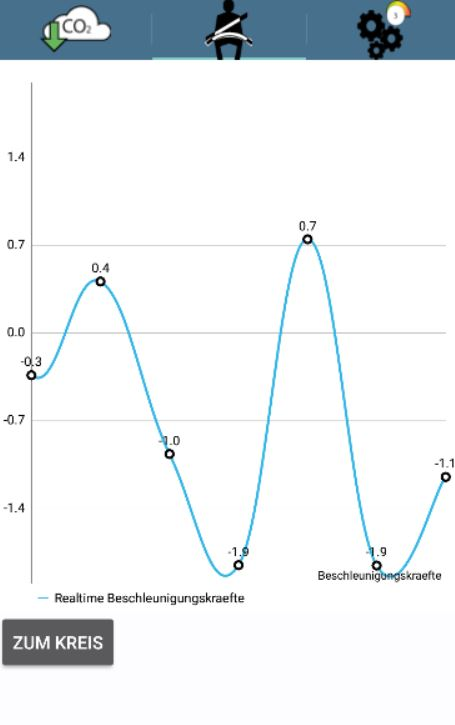
\includegraphics[width=\textwidth]{images/Liniendiagramm}
 		\caption{Längstbeschleunigung mittels MPAndroidChart}
 	\end{minipage}
 	\hfill
 	\begin{minipage}[b]{0.4\textwidth}
 		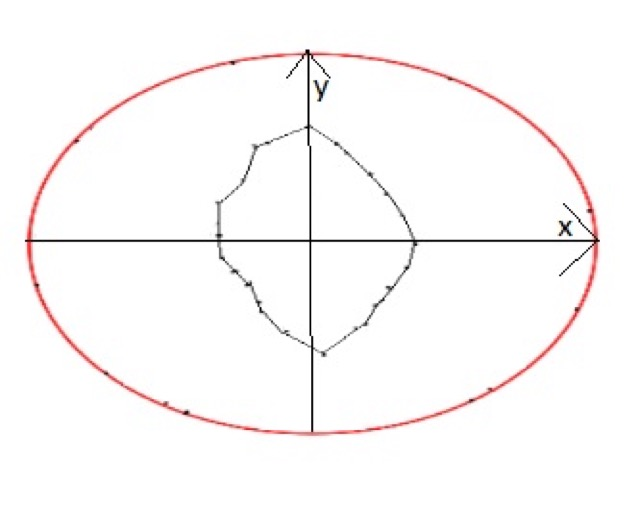
\includegraphics[width=\textwidth]{images/Kammscherkreis-u}
 		\caption{Kammscher Kreis mittels ondraw() - canvas}
 	\end{minipage}
\end{figure}
<<<<<<< HEAD

Das Liniendiagramm stellt die Längstbeschleunigungen da, wobei die Grenzen hierbei von 1.6 bis -1.6 g sind.
Bei der anderen Abbildung kann ein Kammscher-Kreis betrachtet werden, wobei hier die einzelnen Punkte miteinander verbunden wurden und somit eine Grafik entsteht welche anzeigt, dass auf der x-Achse sehr viel Beschleunigt wurde.

=======
 
>>>>>>> aca00159eb7a63f092a2c4b8c38e908b9a2a051b
\clearpage % DO NOT REMOVE